\chapter{Design}

%You may also put some code snippet (which is NOT float by default), eg: \cref{lst:random-code}.

%\lstinputlisting[float,language=Java,label={lst:random-code}]{listings/HelloWorld.java}

\section{Architettura generale client web}
In questa sezione viene esplorato come l'interfaccia web interagisce con le \ac{API} GraphQL per effettuare operazioni sul server e per poi usare i risultati di suddette operazioni per mostrarli graficamente. Nella figura \ref{fig:general-client-architecture-graphics} vengono mostrate le principali componenti protagoniste di questo meccanismo. Le descriviamo in questo modo:

 \begin{itemize}
	\item \textbf{Client Application}: questo \textit{package} contiene tutte le componenti grafiche che vengono rappresentate all'interno della pagina principale. Ogni componente, una volta che l'applicativo viene avviato, è tradotto al browser in formato HTML.
	\item \textbf{ClientConnection}: punto di accesso attraverso il quale è possibile effettuare tutte le operazioni definite secondo lo schema GraphQL. 
	\item \textbf{SimulationControlApi}: questo oggetto contiene tutte le funzioni necessarie a controllare lo stato della simulazione e dipende strettamente dalla componente \textbf{ClientConnection}. Si parla quindi di funzioni utili all'avvio, alla sospensione e terminazione della simulazione. Notare come queste siano tutte operazioni di tipo \textit{mutation}.
	\item \textbf{EnvironmentApi}: è l'oggetto utile a recuperare le informazioni riguardanti un nodo, lo stato \textit{attuale} dell'\textit{Environment}, ma soprattutto utile a recuperare la posizione dei nodi in tempo reale, quindi attraverso l'utilizzo di una \textit{subscription}. 
	\item \textbf{GeneratedModel}: questo pacchetto contiene tutte le risorse generate a partire dallo schema GraphQL esposto dal server. È utilizzato dagli oggetti \textbf{EnvironmentApi} e \textbf{SimulationControlApi} nell'utilizzo dei tipi di dato corretto durante l'utilizzo delle operazioni sul server.
 \end{itemize}

\begin{figure}[htb]
	\centering
	\includegraphics[scale=0.5]{imgs/General_Architecture_Web_Client.pdf}
	\caption{Architettura generale del client web}
	\label{fig:general-client-architecture-graphics}
\end{figure}

Gli oggetti \textbf{SimulationControlApi} e \textbf{EnvironmentApi} sono stati implementati attraverso il design pattern \textit{Singleton}~\cite{Gamma1994}. Sebbene quest'ultimo, se abusato o implementato in modo non adeguato sia considerato di fatto un ``anti-pattern'' \footnote{\url{https://code.google.com/archive/p/google-singleton-detector/wikis/WhySingletonsAreControversial.wiki}}, in questa situazione risulta essere molto comodo, specialmente considerando la necessità di un unico punto di accesso comune al client che effettua le query sul server. Risulterebbe infatti inutile, per ogni componente grafico che ne necessita, istanziare un'altro client GraphQL dal quale effettuare query. Lo stesso vale anche nell'ipotesi in cui vengano utilizzate delle proprietà che fungono da parametri di configurazione dell'applicativo. Un \textit{Singleton} può fornire un punto centralizzato per queste impostazioni.

\section{}


\section{Layout dell'interfaccia}
Il layout dell'interfaccia grafica è stato pensato per rappresentare nel modo più semplice ed intuitivo l'ambiente della simulazione.  La figura \ref{fig:interface-layout} rappresenta un mockup utilizzato durante la fase di progettazione dell'interfaccia. Si possono individuare le seguenti sezioni:
\begin{itemize}
	\item \textbf{Barra di navigazione}: nella parte alta dell'interfaccia è presente una barra di navigazione contenente il titolo e il pulsante per avviare o mettere in pausa la simulazione, ancorato all'estrema destra. Molte interfacce web moderne presentano questo tipo di elemento come \textit{header} della pagina web principale, inteso come punto centrale dal quale è possibile accedere a tutte le sezioni e funzionalità. Questo fornisce all'interfaccia un punto di espandibilità dell'applicativo, come l'aggiunta di una barra di ricerca o di un menù `detto ad `hamburger''. Sarebbe stato possibile, per esempio, inserire una barra di ricerca per i nodi, filtrandoli per categorie di proprietà. Questo tipo di funzionalità è indirizzato a lavori futuri. 
	\item \textbf{Canvas grafico}: la sezione principale di questa interfaccia. All'interno di un contesto grafico bidimensionale vengono rappresentati i nodi della simulazione. Ogni nodo è rappresentato come un cerchio pieno, avente centro le coordinate del nodo e raggio un valore variabile che può essere impostato dall'utente nella sezione descritta successivamente. Lo spazio bidimensionale ha come sfondo una griglia, che  fornisce un riferimento visivo e un aiuto all'orientamento. Funzionalità non banale di questa sezione è che l'utente può spostare il contesto visivo trascinando il cursore sullo schermo, oltre che a effettuare un ingrandimento o una diminuzione della scala. Per ottenere questo tipo di comportamenti sono stati adottati meccanismi ad hoc per il calcolo dello spostamento del \textit{drag} e dello \textit{zoom-in}/\textit{zoom-out}.
	\item \textbf{Informazioni e controlli sul canvas}: in questa sezione vengono raccolte le principali informazioni riguardo al contesto come il fattore di \textit{zoom} corrente, la differenza di traslazione rispetto all'origine e lo \textit{slider} per il cambiamento del raggio dei nodi.
	\item \textbf{Sezione di ispezione di un nodo}: qui vengono rappresentate tutte le informazioni riguardanti un nodo. Sono presenti quindi il codice identificativo, posizione nello spazio bidimensionale, proprietà, i contenuti (intesi come una mappa che ha come chiavi le molecole e  valori le relative concentrazioni), e le reazioni (Vedi \ref{label}). Per le ultime tre categorie sono stati usati degli elementi che possono essere ``collassati'' in quanto non è garantito che queste proprietà siano presenti (sempre per il fatto che \textit{Alchemist} può rappresentare una certa gamma di simulazioni tra loro eterogenee).
\end{itemize}

\begin{figure}[htb]
	\centering
	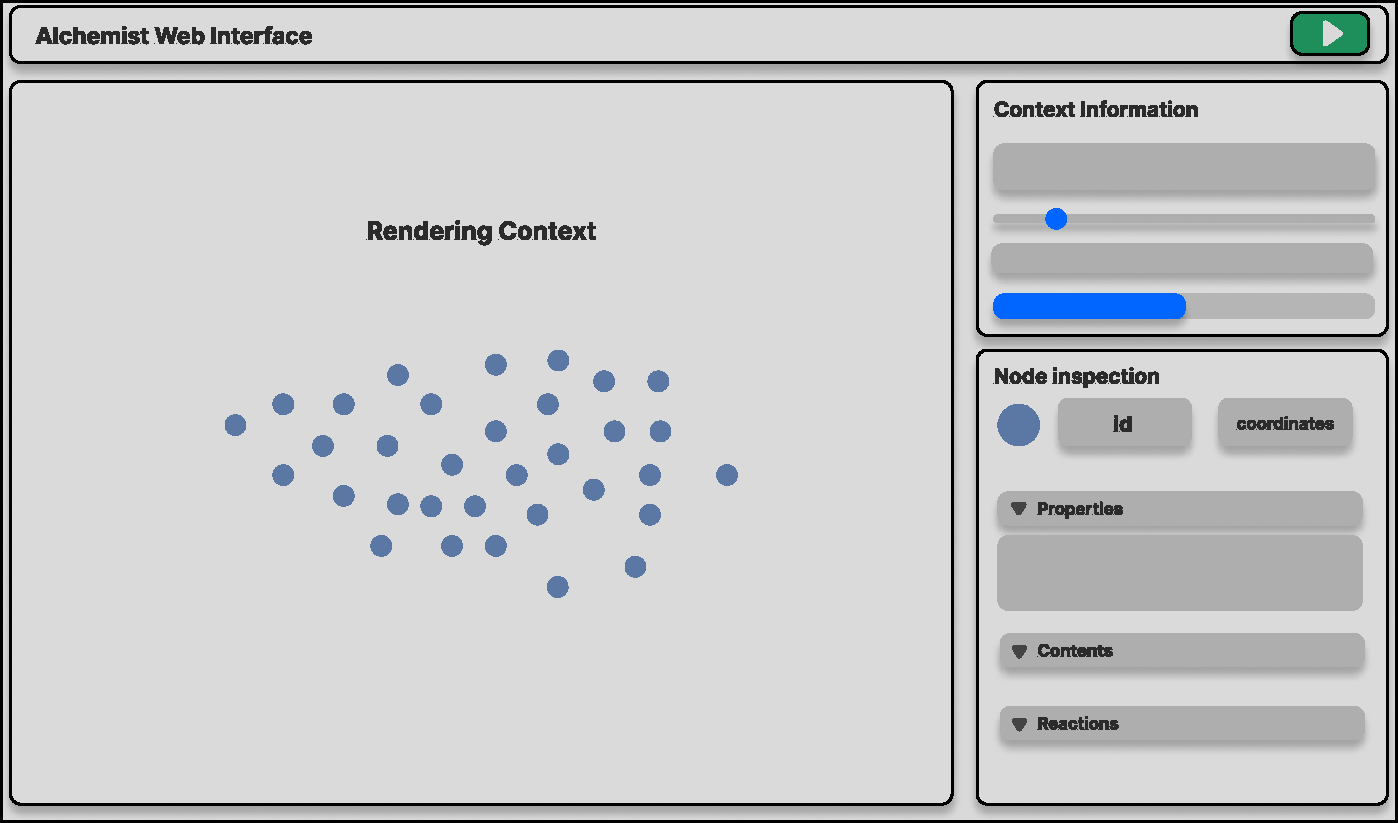
\includegraphics[scale=0.65]{imgs/Interface_Layout.pdf}
	\caption{Mockup dell'interfaccia grafica}
	\label{fig:interface-layout}
\end{figure}

